

\subsection{Distribution of events}
\begin{figure} [H]
    \centering
    \caption{Distribution of events}
    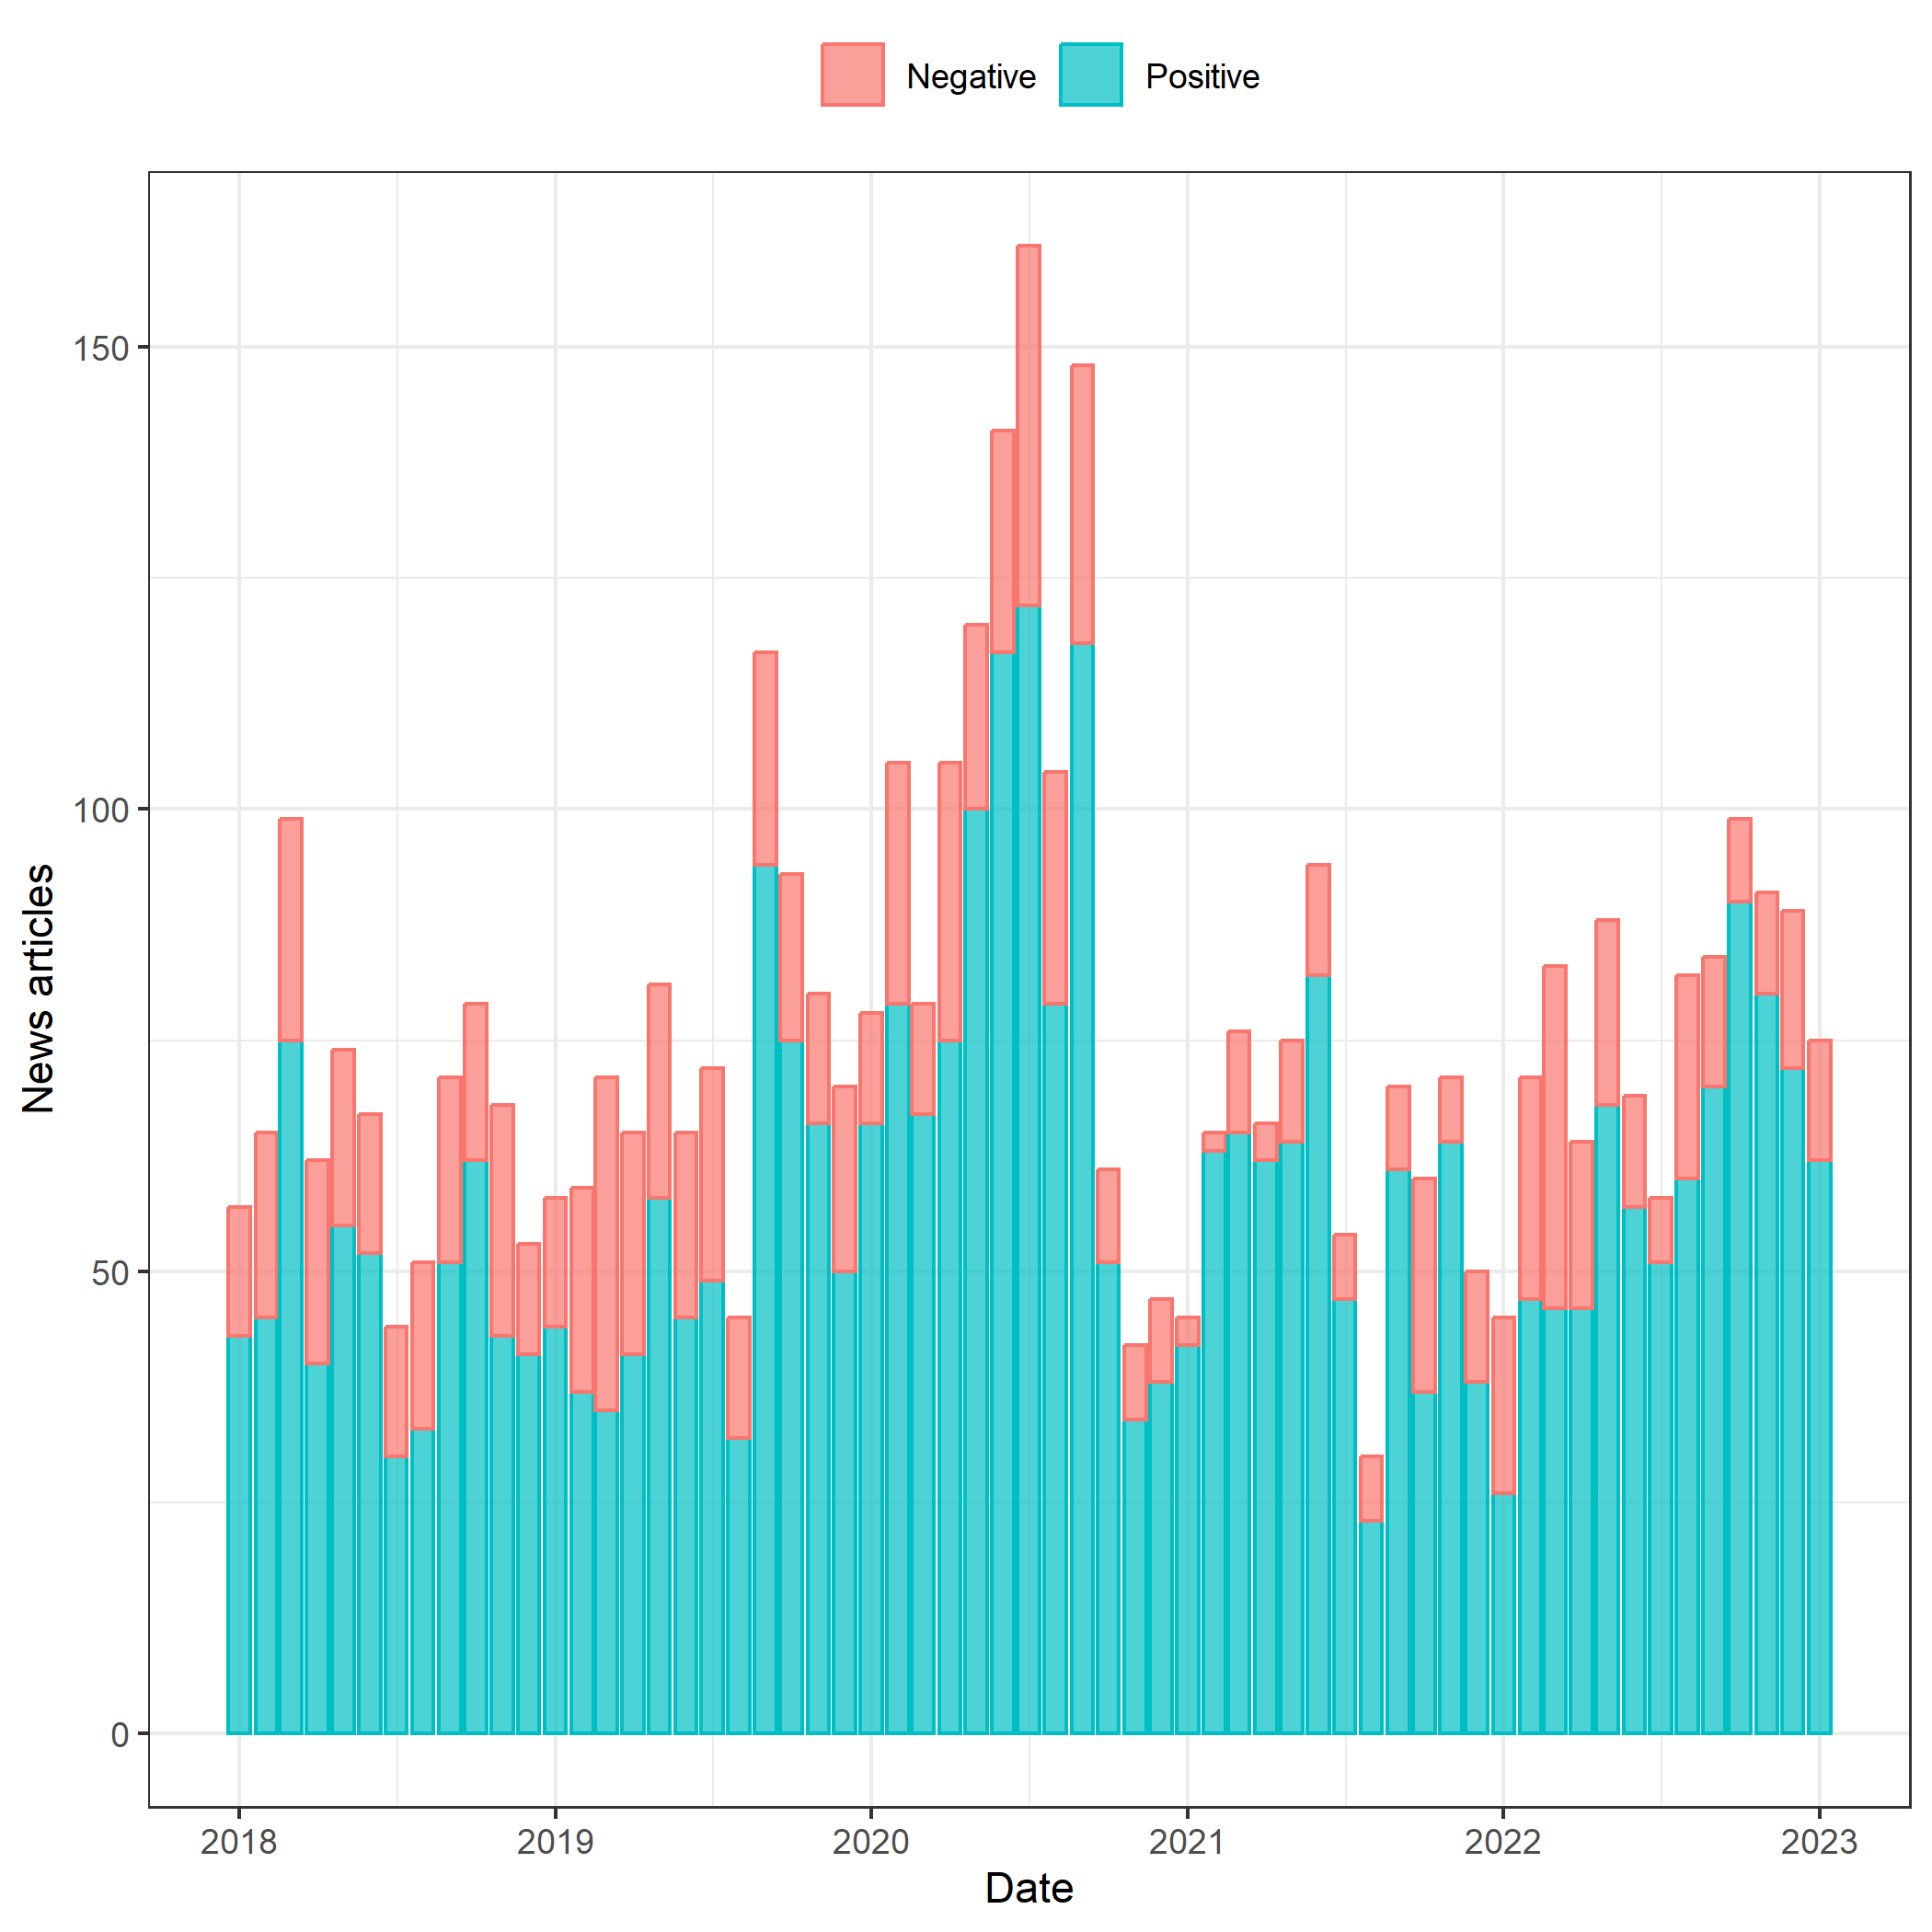
\includegraphics[scale=0.5]{Projekt/1.Figures analysis/event_distribution.png}
    \label{fig:event_distribution}
\end{figure}

\begin{figure} [H]
    \centering
    \caption{Distribution of events per SDG}
    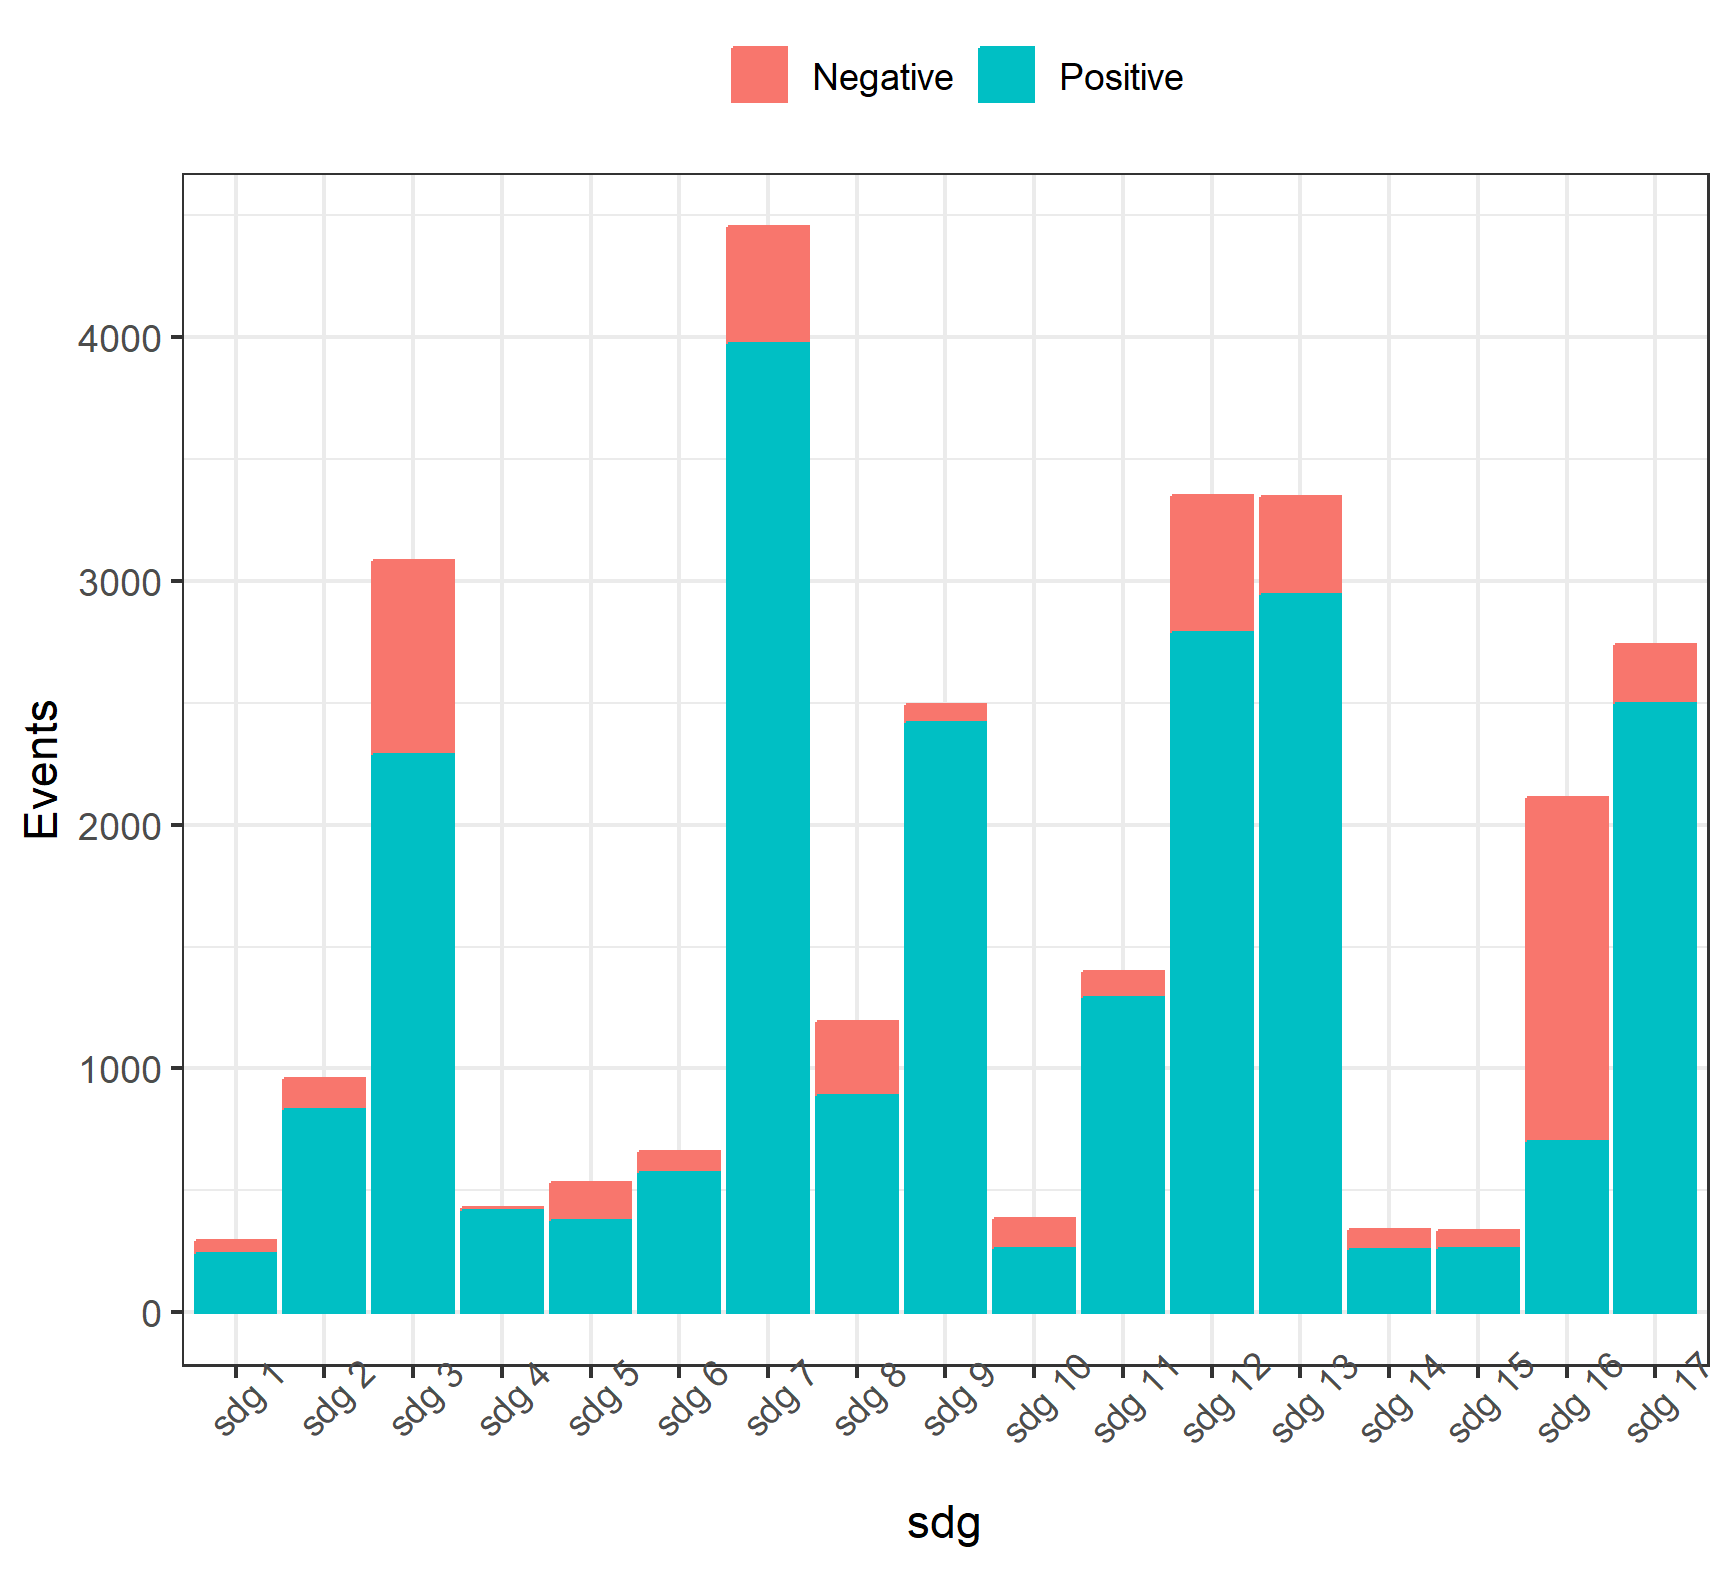
\includegraphics[scale=0.5]{Projekt/1.Figures analysis/event_distribution_SDG.png}
    \label{fig:event_distribution_SDG}
\end{figure}

\subsection{Empirical results}

\begin{figure} [H]
    \centering
    \caption{Negative news: AAR split on relation to SDGs}
    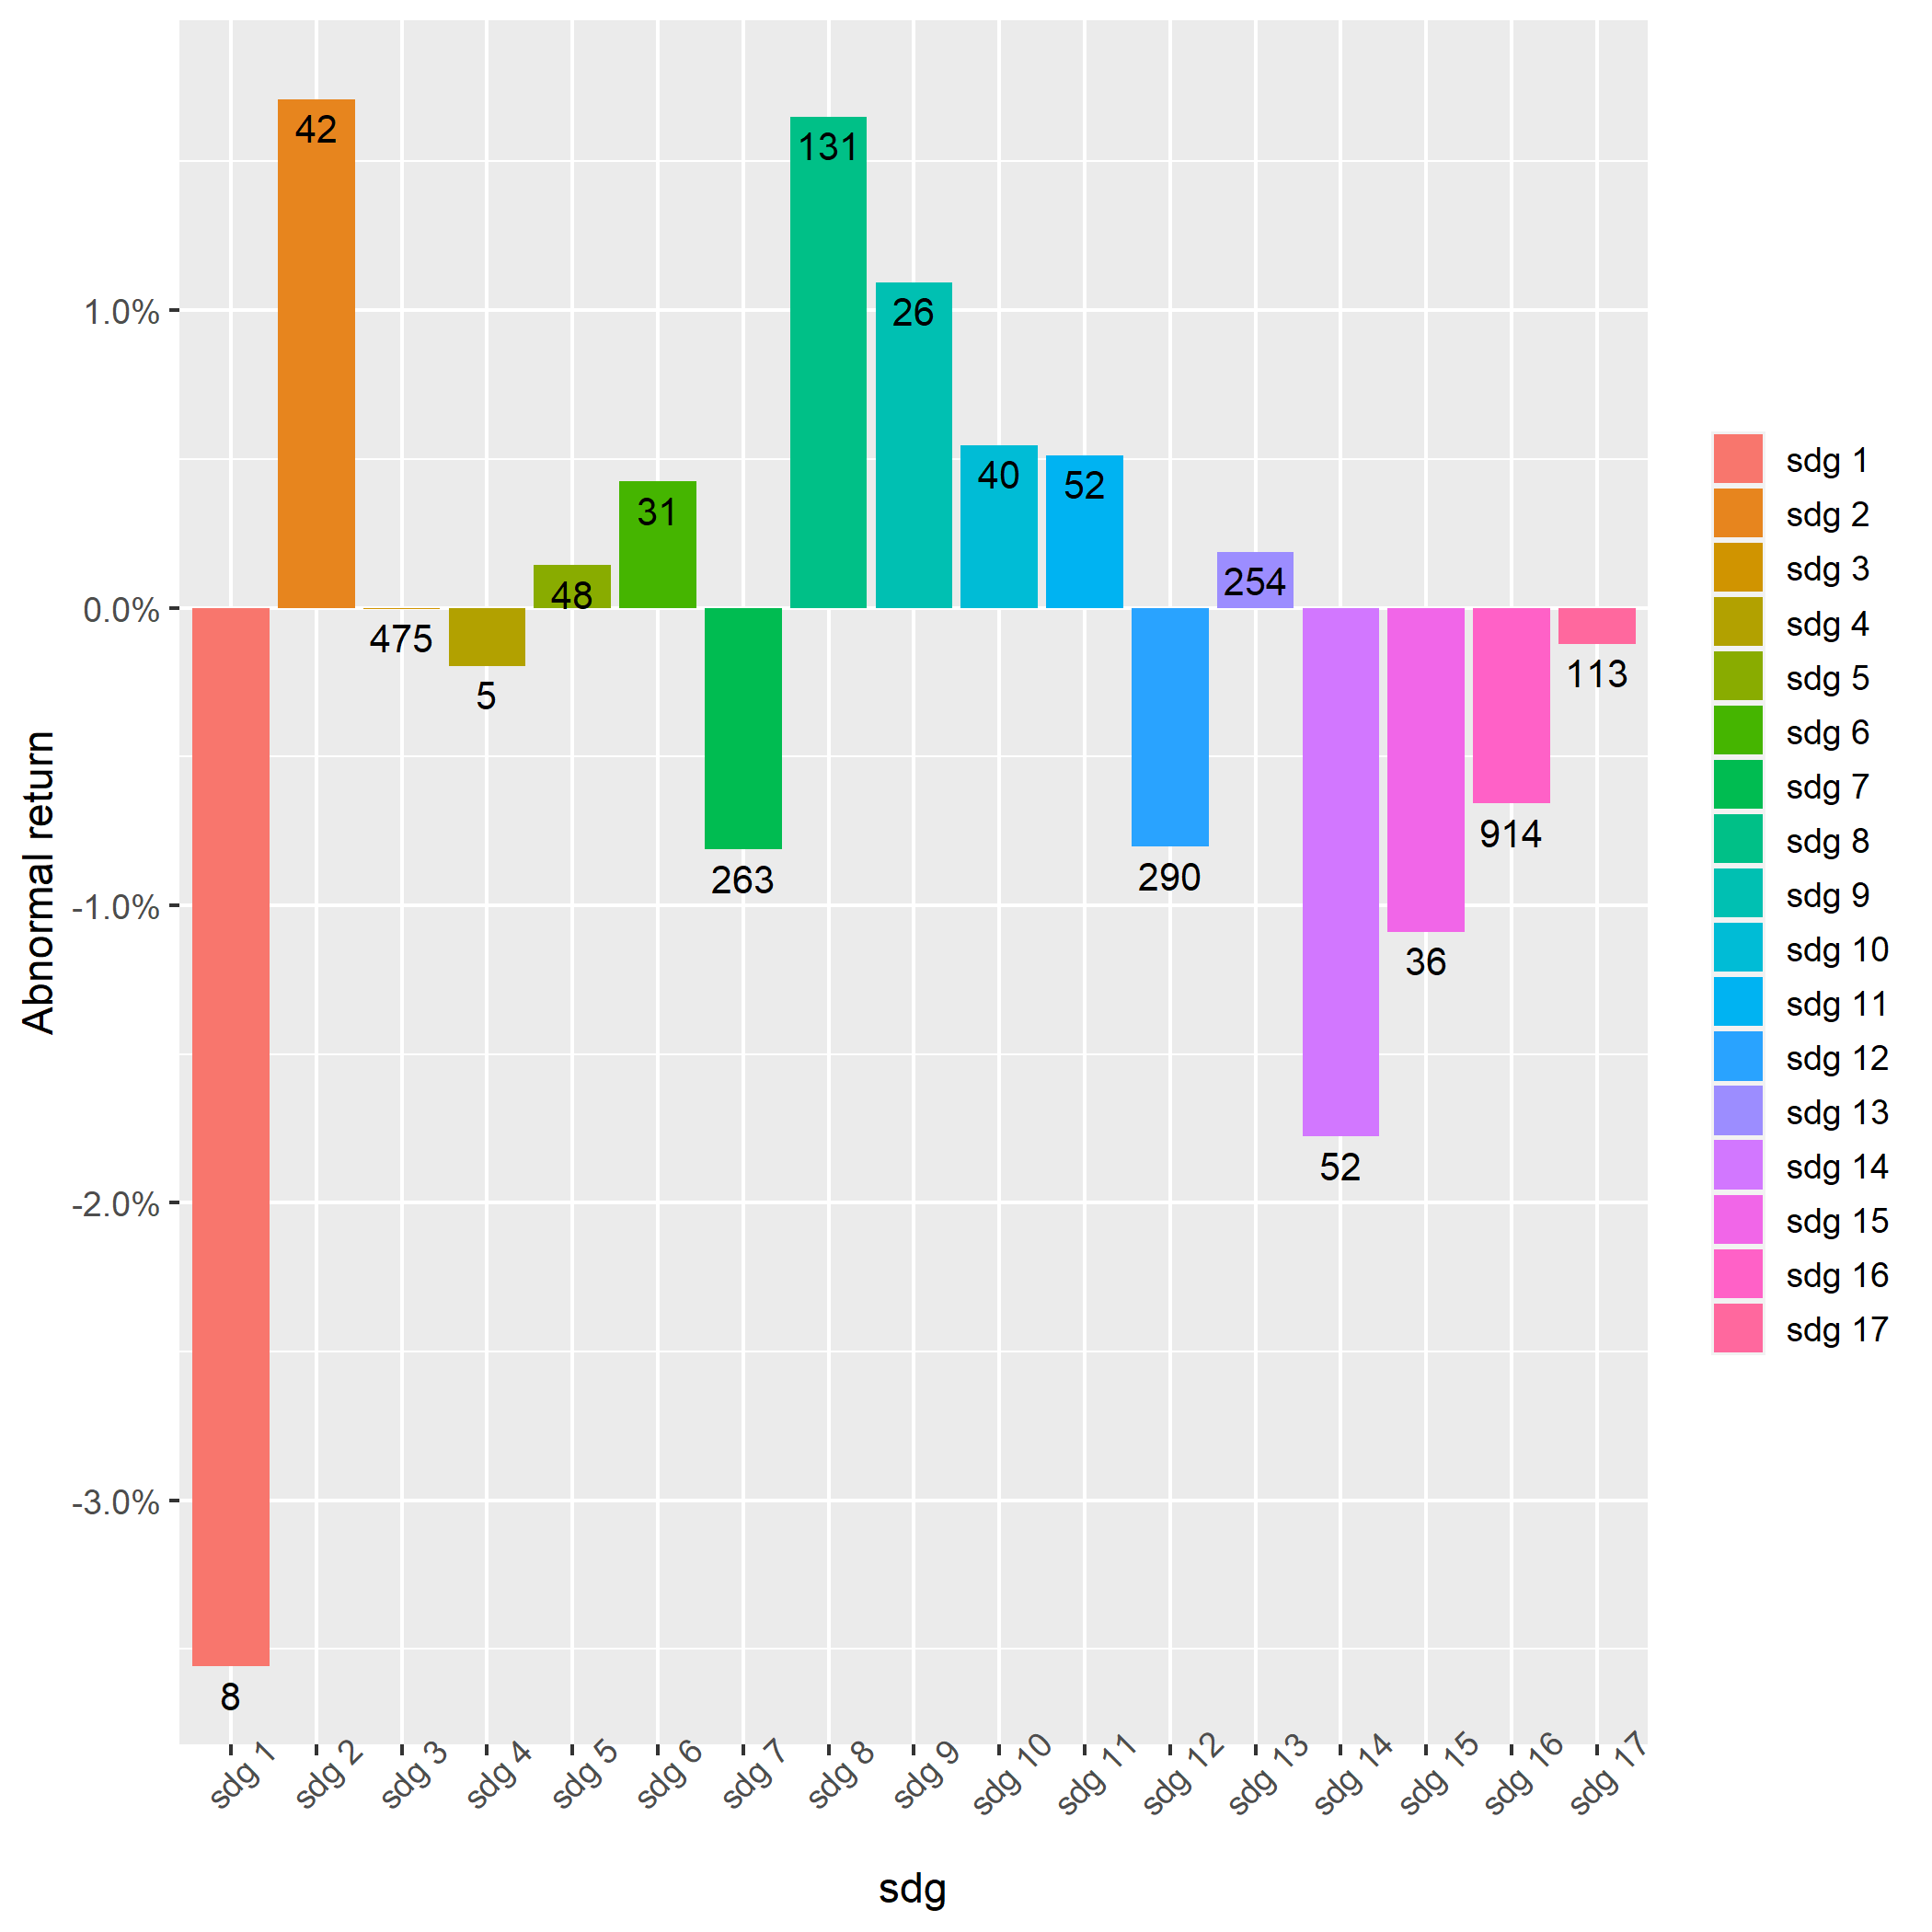
\includegraphics[scale=0.5]{Projekt/1.Figures analysis/ST_negative_sdg_bar.png}
    \caption*{\footnotesize The figure illustrates the CAAR on $t = 10$ from negative news. The error bars represent the 95\% confidence intervals of the AAR.}
    \label{fig:ST_neg_bar_all}
\end{figure}

\begin{figure} [H]
    \centering
    \caption{AAR per SDG: positive news}
    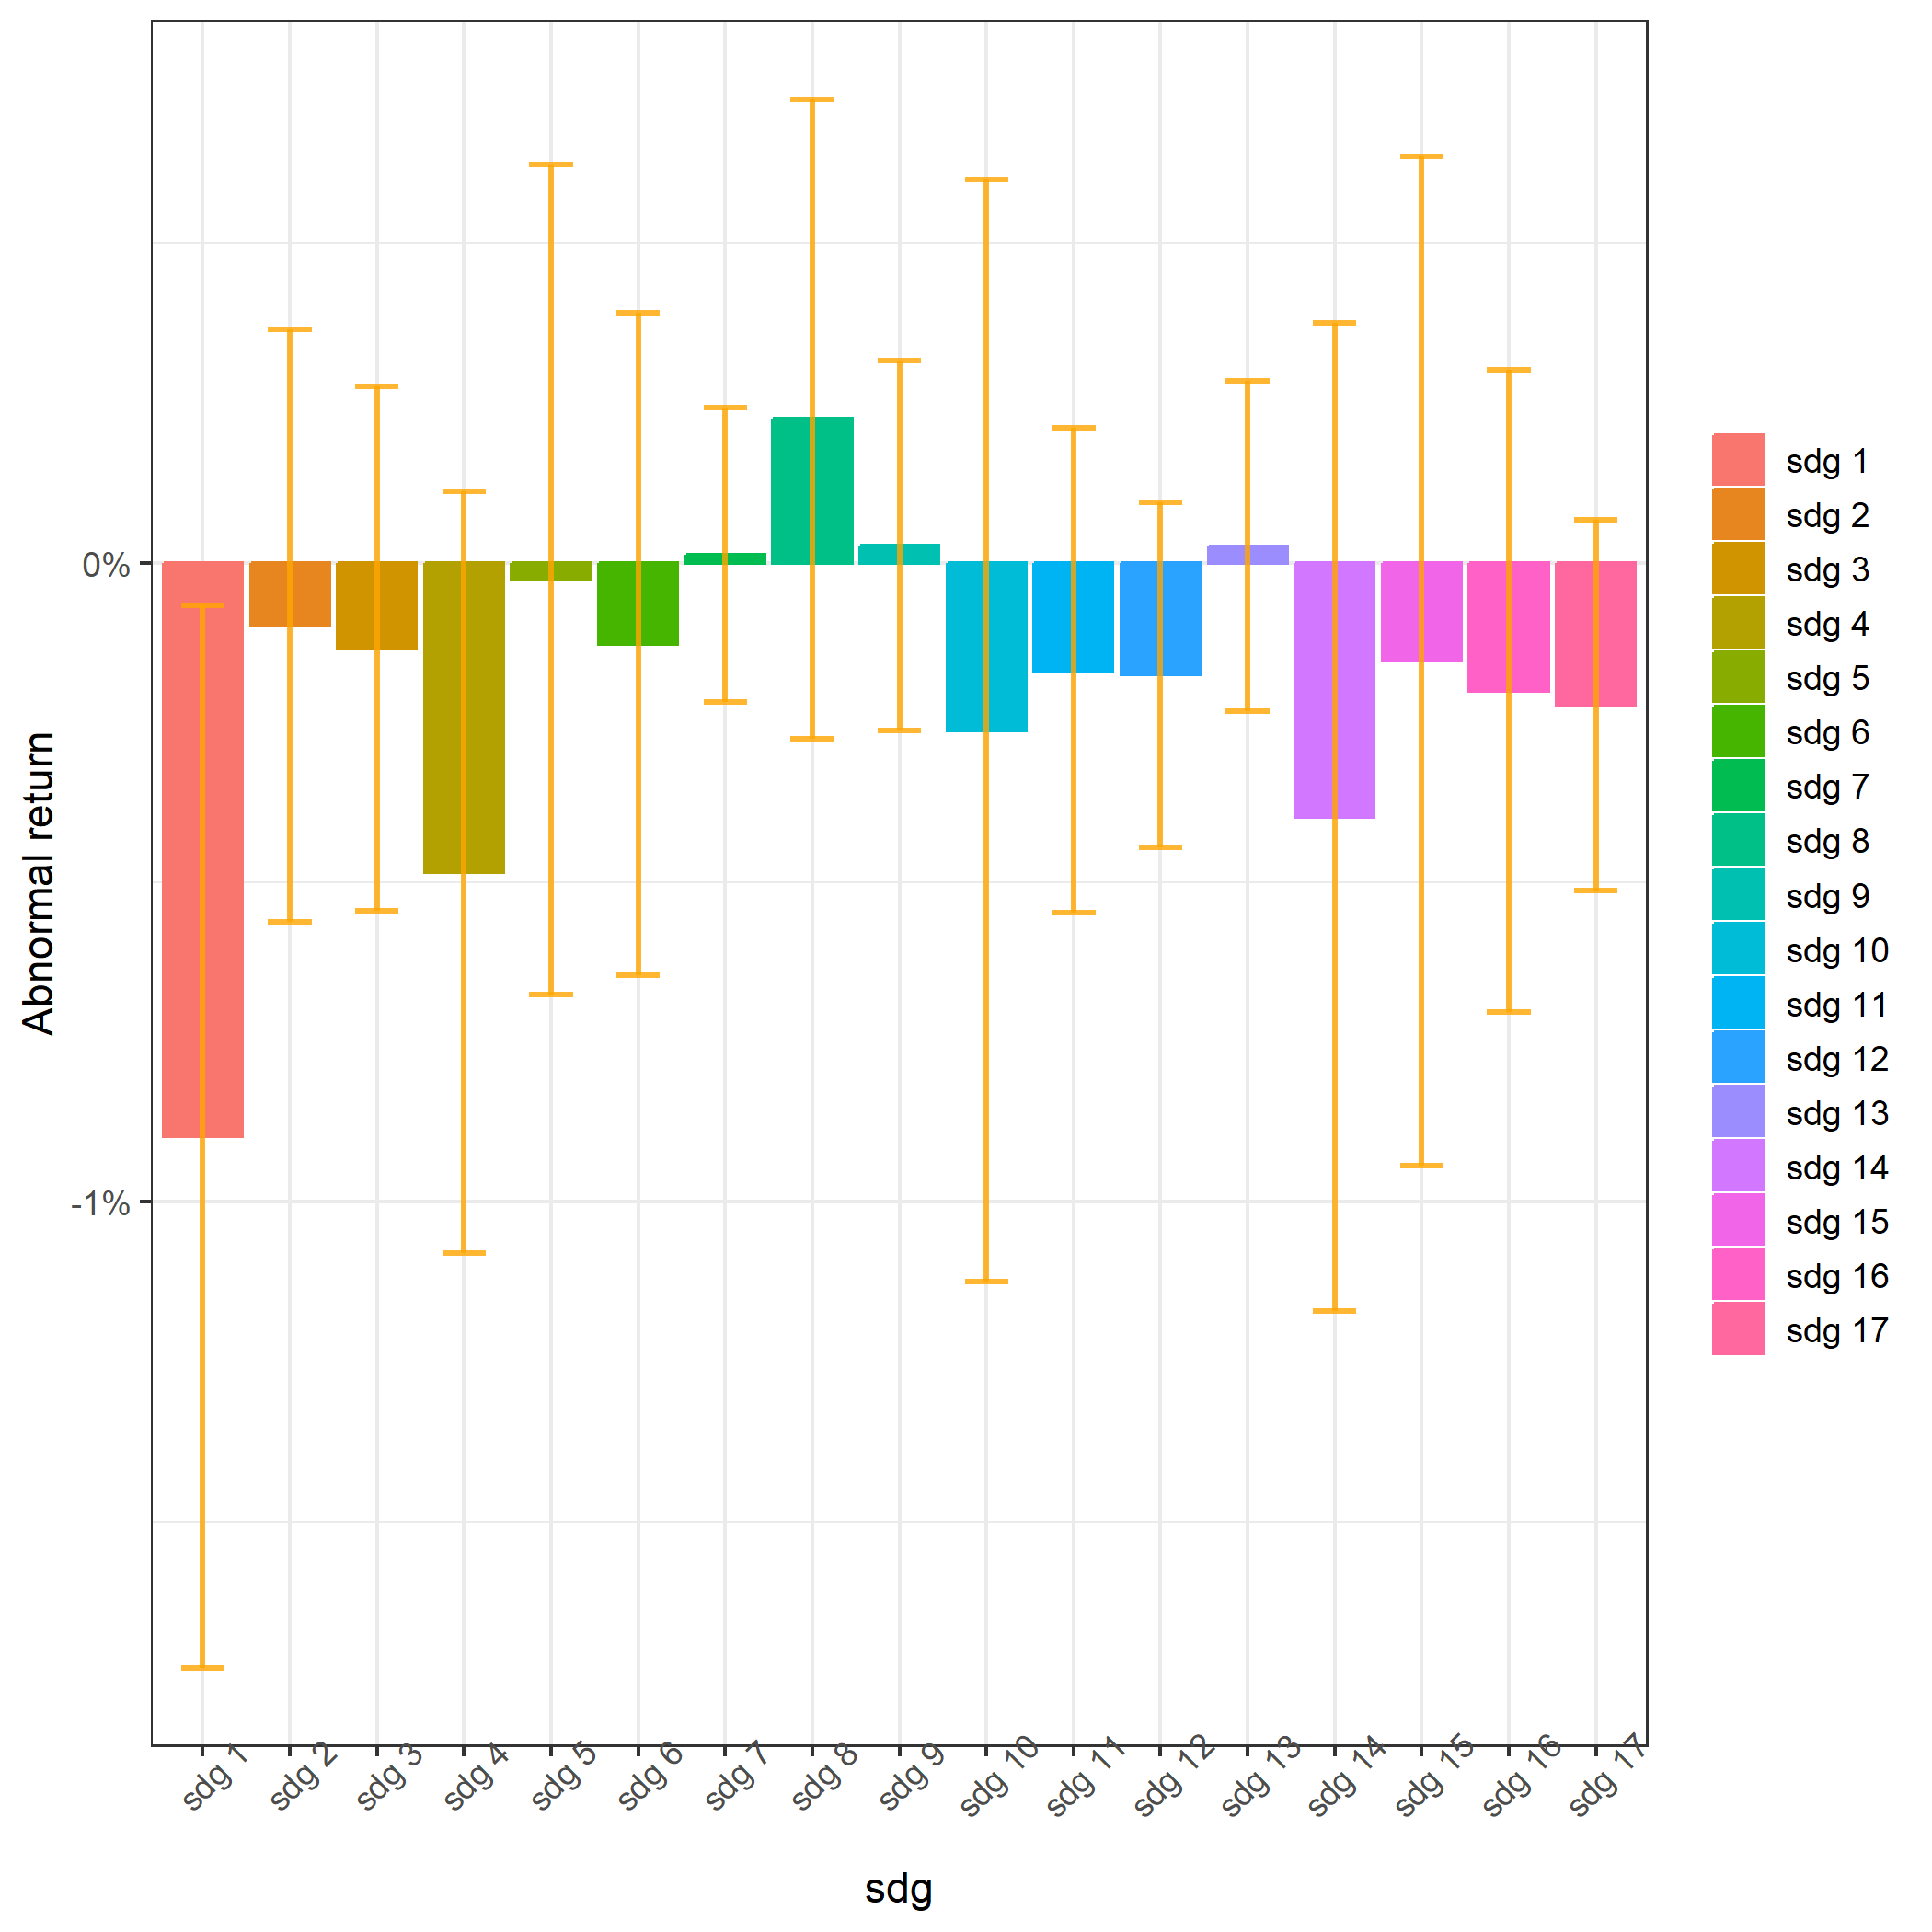
\includegraphics[scale=0.5]{Projekt/1.Figures analysis/ST_positive_sdg_bar.png}
    \caption*{\footnotesize The figure illustrates the CAAR on $t = 10$ from positive news. The error bars represent the 95\% confidence intervals of the AAR.}
    \label{fig:ST_pos_bar_all}
\end{figure}

\subsubsection{Long-term regression statistics}
% latex table generated in R 4.2.2 by xtable 1.8-4 package
% Wed May 10 16:49:08 2023
\begin{table}[H]
\centering
\caption{Regression summary: Negative news, SD = 1} 
\begin{tabular}{lrrrr}
  \hline
term & estimate & std.error & statistic & p.value \\ 
  \hline
(Intercept) & -0.0084 & 0.0028 & -2.9668 & 0.0045 \\ 
  mkt\_excess\_ret & 1.1580 & 0.0752 & 15.3975 & 0.0000 \\ 
  SMB & -0.0404 & 0.1761 & -0.2295 & 0.8194 \\ 
  HML & 0.3102 & 0.1960 & 1.8824 & 0.0763 \\ 
  RMW & -0.0785 & 0.2963 & -0.2648 & 0.7922 \\ 
  CMA & -0.1652 & 0.2975 & -0.5554 & 0.5809 \\ 
   \hline
\end{tabular}
\label{tab: summary_neg_1}
\end{table}



% latex table generated in R 4.2.2 by xtable 1.8-4 package
% Wed May 10 16:49:21 2023
\begin{table}[ht]
\centering
\begin{tabular}{lrrrr}
  \hline
term & estimate & std.error & statistic & p.value \\ 
  \hline
(Intercept) & -0.0036 & 0.0016 & -2.2323 & 0.0298 \\ 
  mkt\_excess\_ret & 1.1057 & 0.0416 & 26.5749 & 0.0000 \\ 
  SMB & -0.2685 & 0.0999 & -2.6868 & 0.0096 \\ 
  HML & -0.0524 & 0.1138 & -0.4607 & 0.6469 \\ 
  RMW & -0.2248 & 0.1714 & -1.3120 & 0.1951 \\ 
  CMA & 0.1407 & 0.1837 & 0.7662 & 0.4469 \\ 
   \hline
\end{tabular}
\label{tab: summary_neg_2}
\end{table}




% latex table generated in R 4.2.2 by xtable 1.8-4 package
% Wed May 10 17:43:02 2023
\begin{table}[H]
\centering
\caption{Regression summary: Negative news, low ESG risk}
\begin{tabular}{lrrrr}
  \hline
term & estimate & std.error & statistic & p.value \\ 
  \hline
(Intercept) & -0.0065 & 0.0032 & -2.0477 & 0.0455 \\ 
  mkt\_excess\_ret & 1.2045 & 0.0867 & 13.8887 & 0.0000 \\ 
  SMB & -0.2876 & 0.2032 & -1.4157 & 0.1626 \\ 
  HML & -0.2765 & 0.2234 & -1.5775 & 0.0912 \\ 
  RMW & -0.5773 & 0.3311 & -1.7432 & 0.0870 \\ 
  CMA & -0.2368 & 0.3251 & -0.7284 & 0.4695 \\ 
   \hline
\end{tabular}
\label{tab: summary_neg_ESG_L}
\end{table}



% latex table generated in R 4.2.2 by xtable 1.8-4 package
% Thu May 11 17:23:01 2023
\begin{table}[H]
\caption{Regression summary: Negative news, medium ESG risk}
\centering
\begin{tabular}{lrrrr}
  \hline
term & estimate & std.error & statistic & p.value \\ 
  \hline
(Intercept) & -0.0061 & 0.0045 & -1.3512 & 0.1823 \\ 
  mkt\_excess\_ret & 1.1760 & 0.1187 & 9.9089 & 0.0000 \\ 
  SMB & 0.4170 & 0.2800 & 1.4890 & 0.1423 \\ 
  HML & 0.7282 & 0.3135 & 2.3228 & 0.0240 \\ 
  RMW & 0.6120 & 0.4777 & 1.2812 & 0.2056 \\ 
  CMA & 0.2064 & 0.4797 & 0.4303 & 0.6687 \\ 
   \hline
\end{tabular}
\end{table}



% latex table generated in R 4.2.2 by xtable 1.8-4 package
% Wed May 10 18:23:13 2023
\begin{table}[H]
\caption{Regression summary: Negative news, equal weights}
\centering
\begin{tabular}{lrrrr}
  \hline
term & estimate & std.error & statistic & p.value \\ 
  \hline
(Intercept) & -0.0096 & 0.0024 & -3.9377 & 0.0002 \\ 
  mkt\_excess\_ret & 1.2126 & 0.0647 & 18.7381 & 0.0000 \\ 
  SMB & 0.5152 & 0.1516 & 3.3994 & 0.0013 \\ 
  HML & 0.2215 & 0.1687 & 1.3131 & 0.0947 \\ 
  RMW & 0.3105 & 0.2550 & 1.2177 & 0.2286 \\ 
  CMA & 0.1564 & 0.2560 & 0.6109 & 0.5439 \\ 
   \hline
\end{tabular}
\label{tab: summary_neg_EW}
\end{table}



\subsection{Sensitivity analysis figures:} \label{app: sensitivity}

\subsubsection{Short-term}

\begin{figure} [H]
    \centering
    \caption{Positive news: event identification rule}
    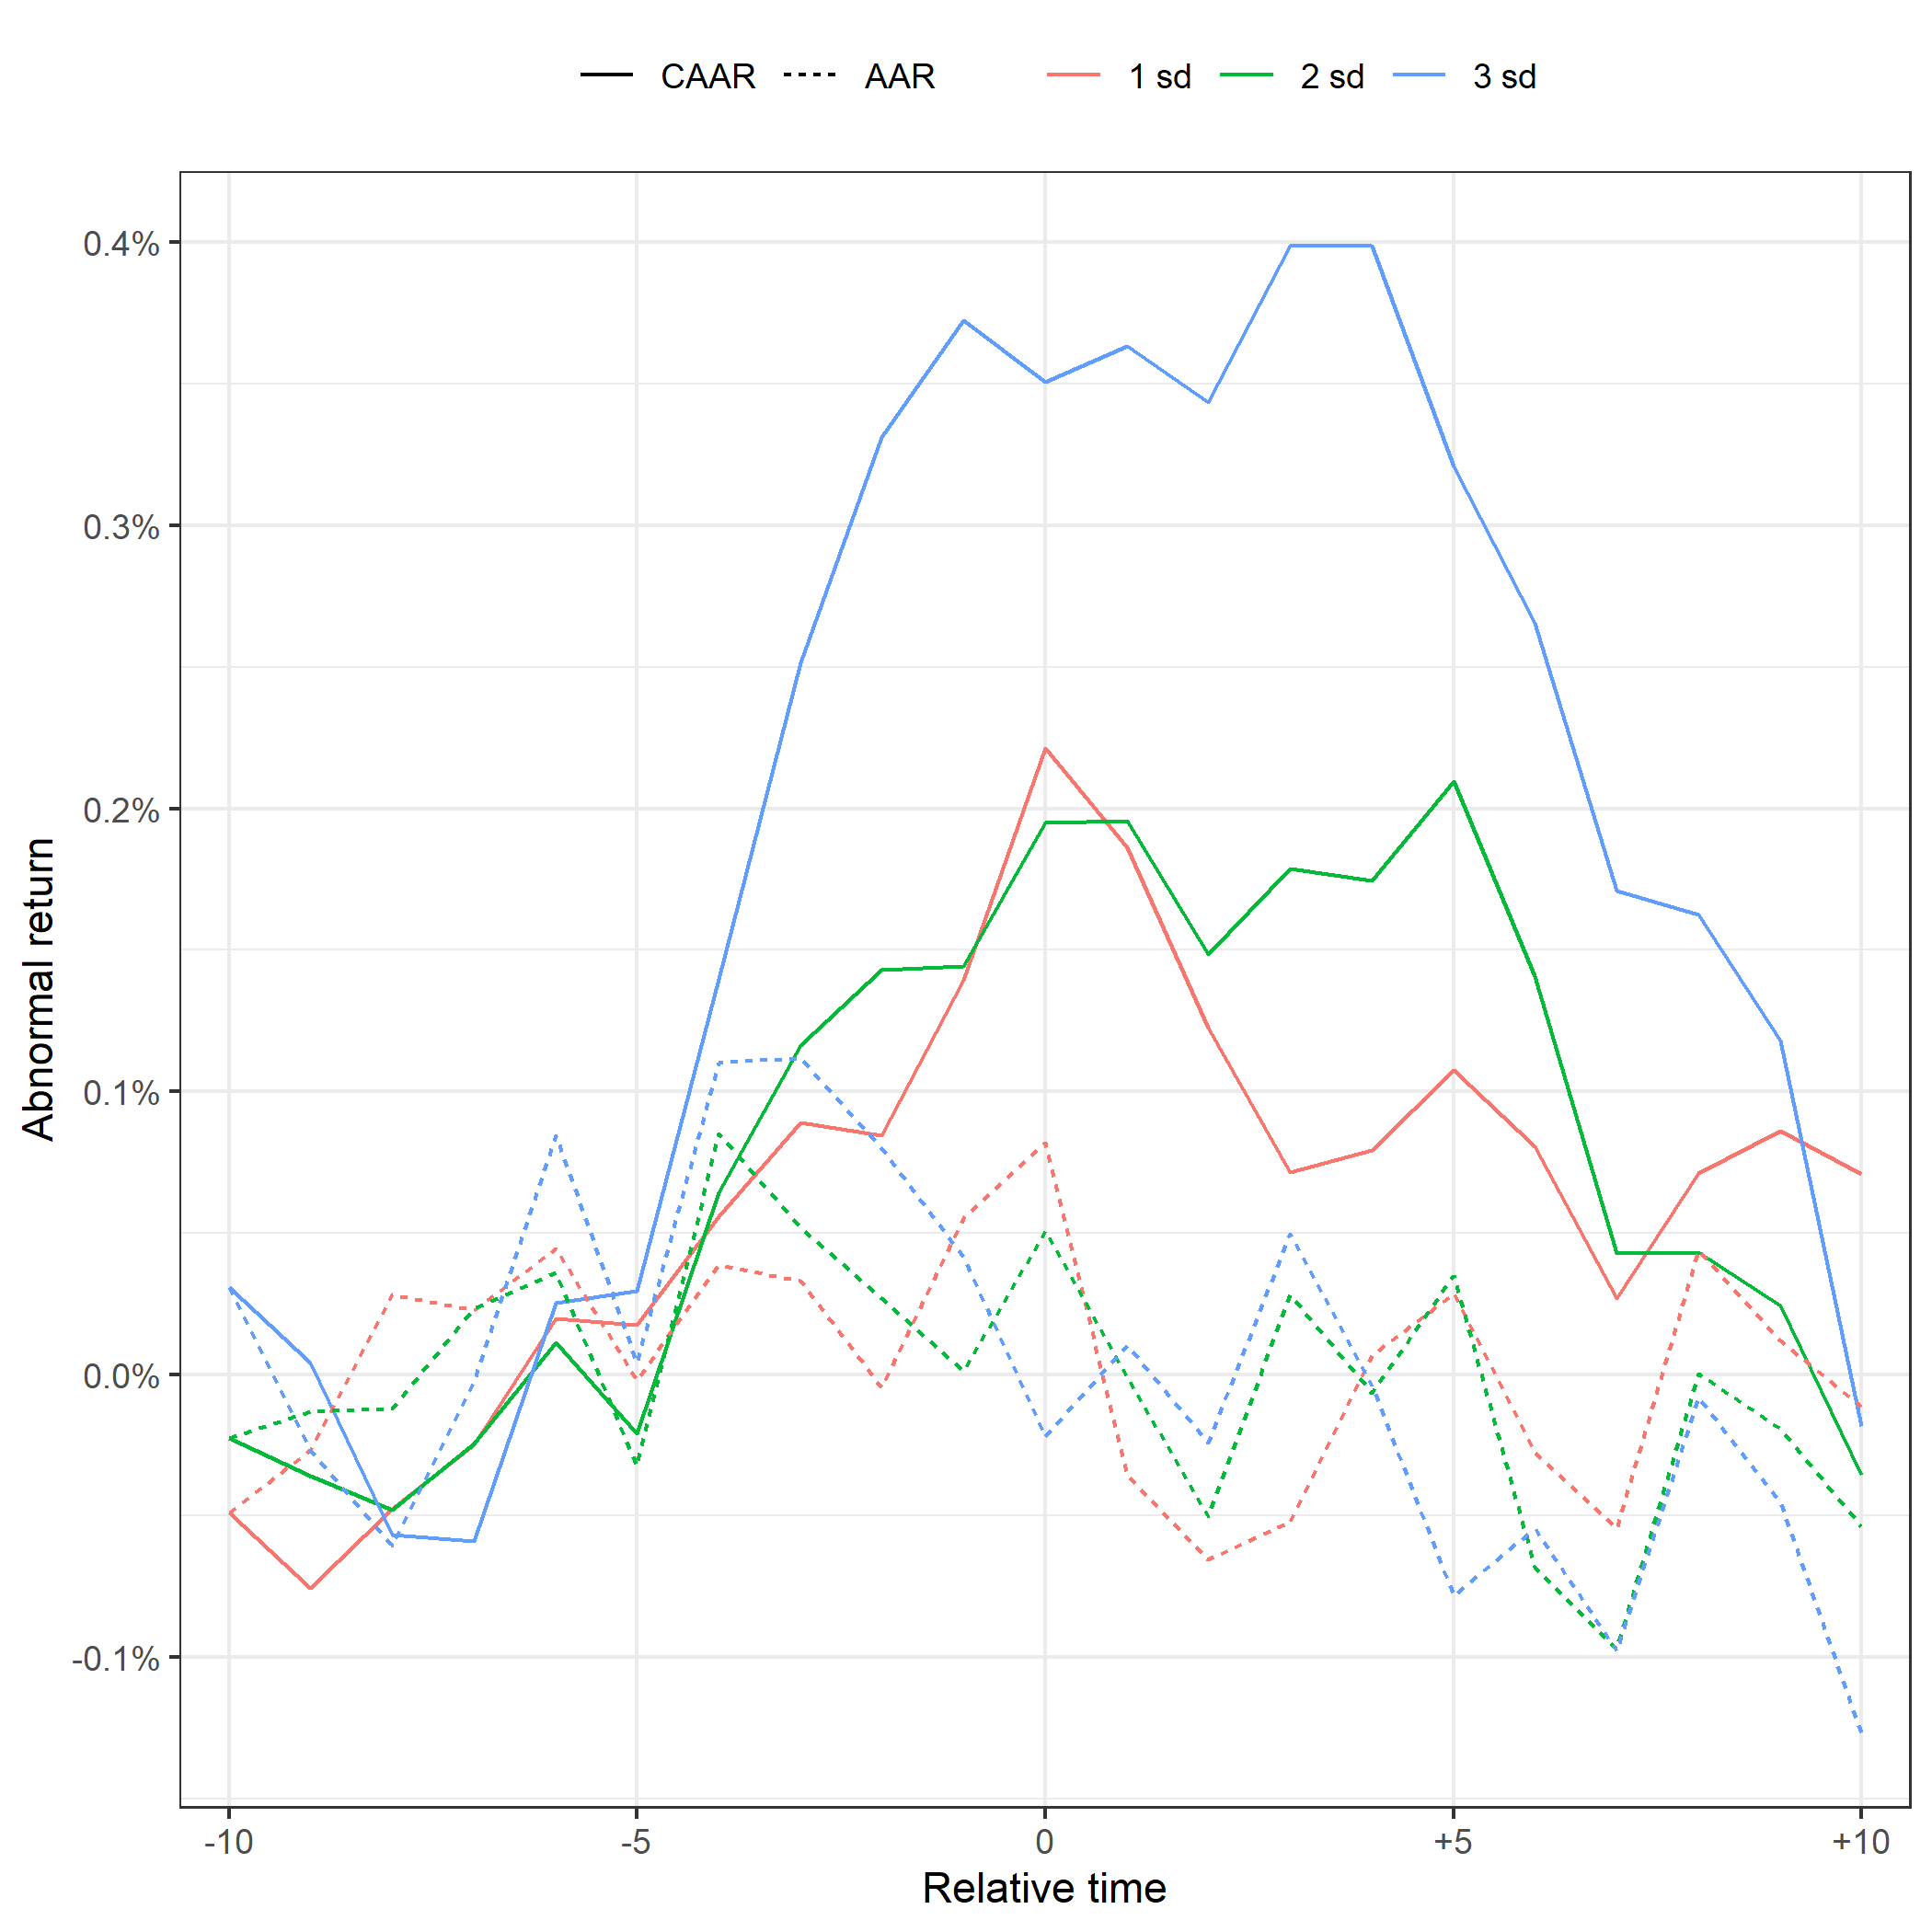
\includegraphics[scale=0.6]{Projekt/1.Figures analysis/ST_positive_sensitivity.png}
     \caption*{\footnotesize The figure illustrates the average abnormal return (AAR) and cumulative AAR (CAAR) around the event date (t = 0) of negative news. The figure illustrates the average abnormal return (AAR) and cumulative AAR (CAAR) around the event date (t = 0) of negative news. The various colors represent whether the event identification rule was based on 1, 2, or 3 standard errors. }
    \label{fig:ST_pos_sensi_sd}
\end{figure} 


\begin{table}[H]
\centering
\caption{AAR and CAAR (in \%) with new event rule (sd)} 
\begin{tabular}{lccccc}
  \hline  \hline
  & \multicolumn{2}{c}{Positive} &  & \multicolumn{2}{c}{Negative}\\ \cline{2-3} \cline{5-6}  
  & 2 sd & 3 sd & & 2 sd & 3 sd   \\   
 \hline
$AAR_{t=0}$ & $\underset{(0.875)}{0.051}$ & $\underset{(-0.278)}{-0.022}$ & & $\underset{(-3.409)}{-0.227^{***}}$ & $\underset{(-3.024)}{-0.210^{***}}$ \\ 
$CAAR_{[-5;+5]}$  & $\underset{(0.283)}{0.031}$  & $\underset{(0.631)}{0.089}$ & & $\underset{(-3.66)}{-0.714^{***}}$ & $\underset{(-2.648)}{-0.657^{***}}$ \\ 
$CAAR_{[-10;+10]}$  & $\underset{(-0.168)}{-0.035}$  & $\underset{(-0.062)}{-0.018}$ &  & $\underset{(-1.886)}{-0.652^{*}}$ & $\underset{(-1.686)}{-0.697^{*}}$  \\
   \hline \hline
   \multicolumn{6}{p{12cm}}{ \footnotesize $^* \; p\; <\; 0.1$, $ ^{**} \; p\; <\; 0.05$, $ ^{***} \; p\; <\; 0.01$  } \\
   \multicolumn{6}{p{13cm}}{\footnotesize The table shows the CAAR associated with positive and negative news over an event window of 5, 10, and 21 days surrounding the event date along with the AAR on $t=0$. The models are split on the requirement rule for included events (2 or 3 sd).} \\
   \hline
\end{tabular}
\label{tab:ST_sensitivity}
\end{table}

\begin{figure} [H]
    \centering
    \caption{Positive news: Value vs. Equal weights}
    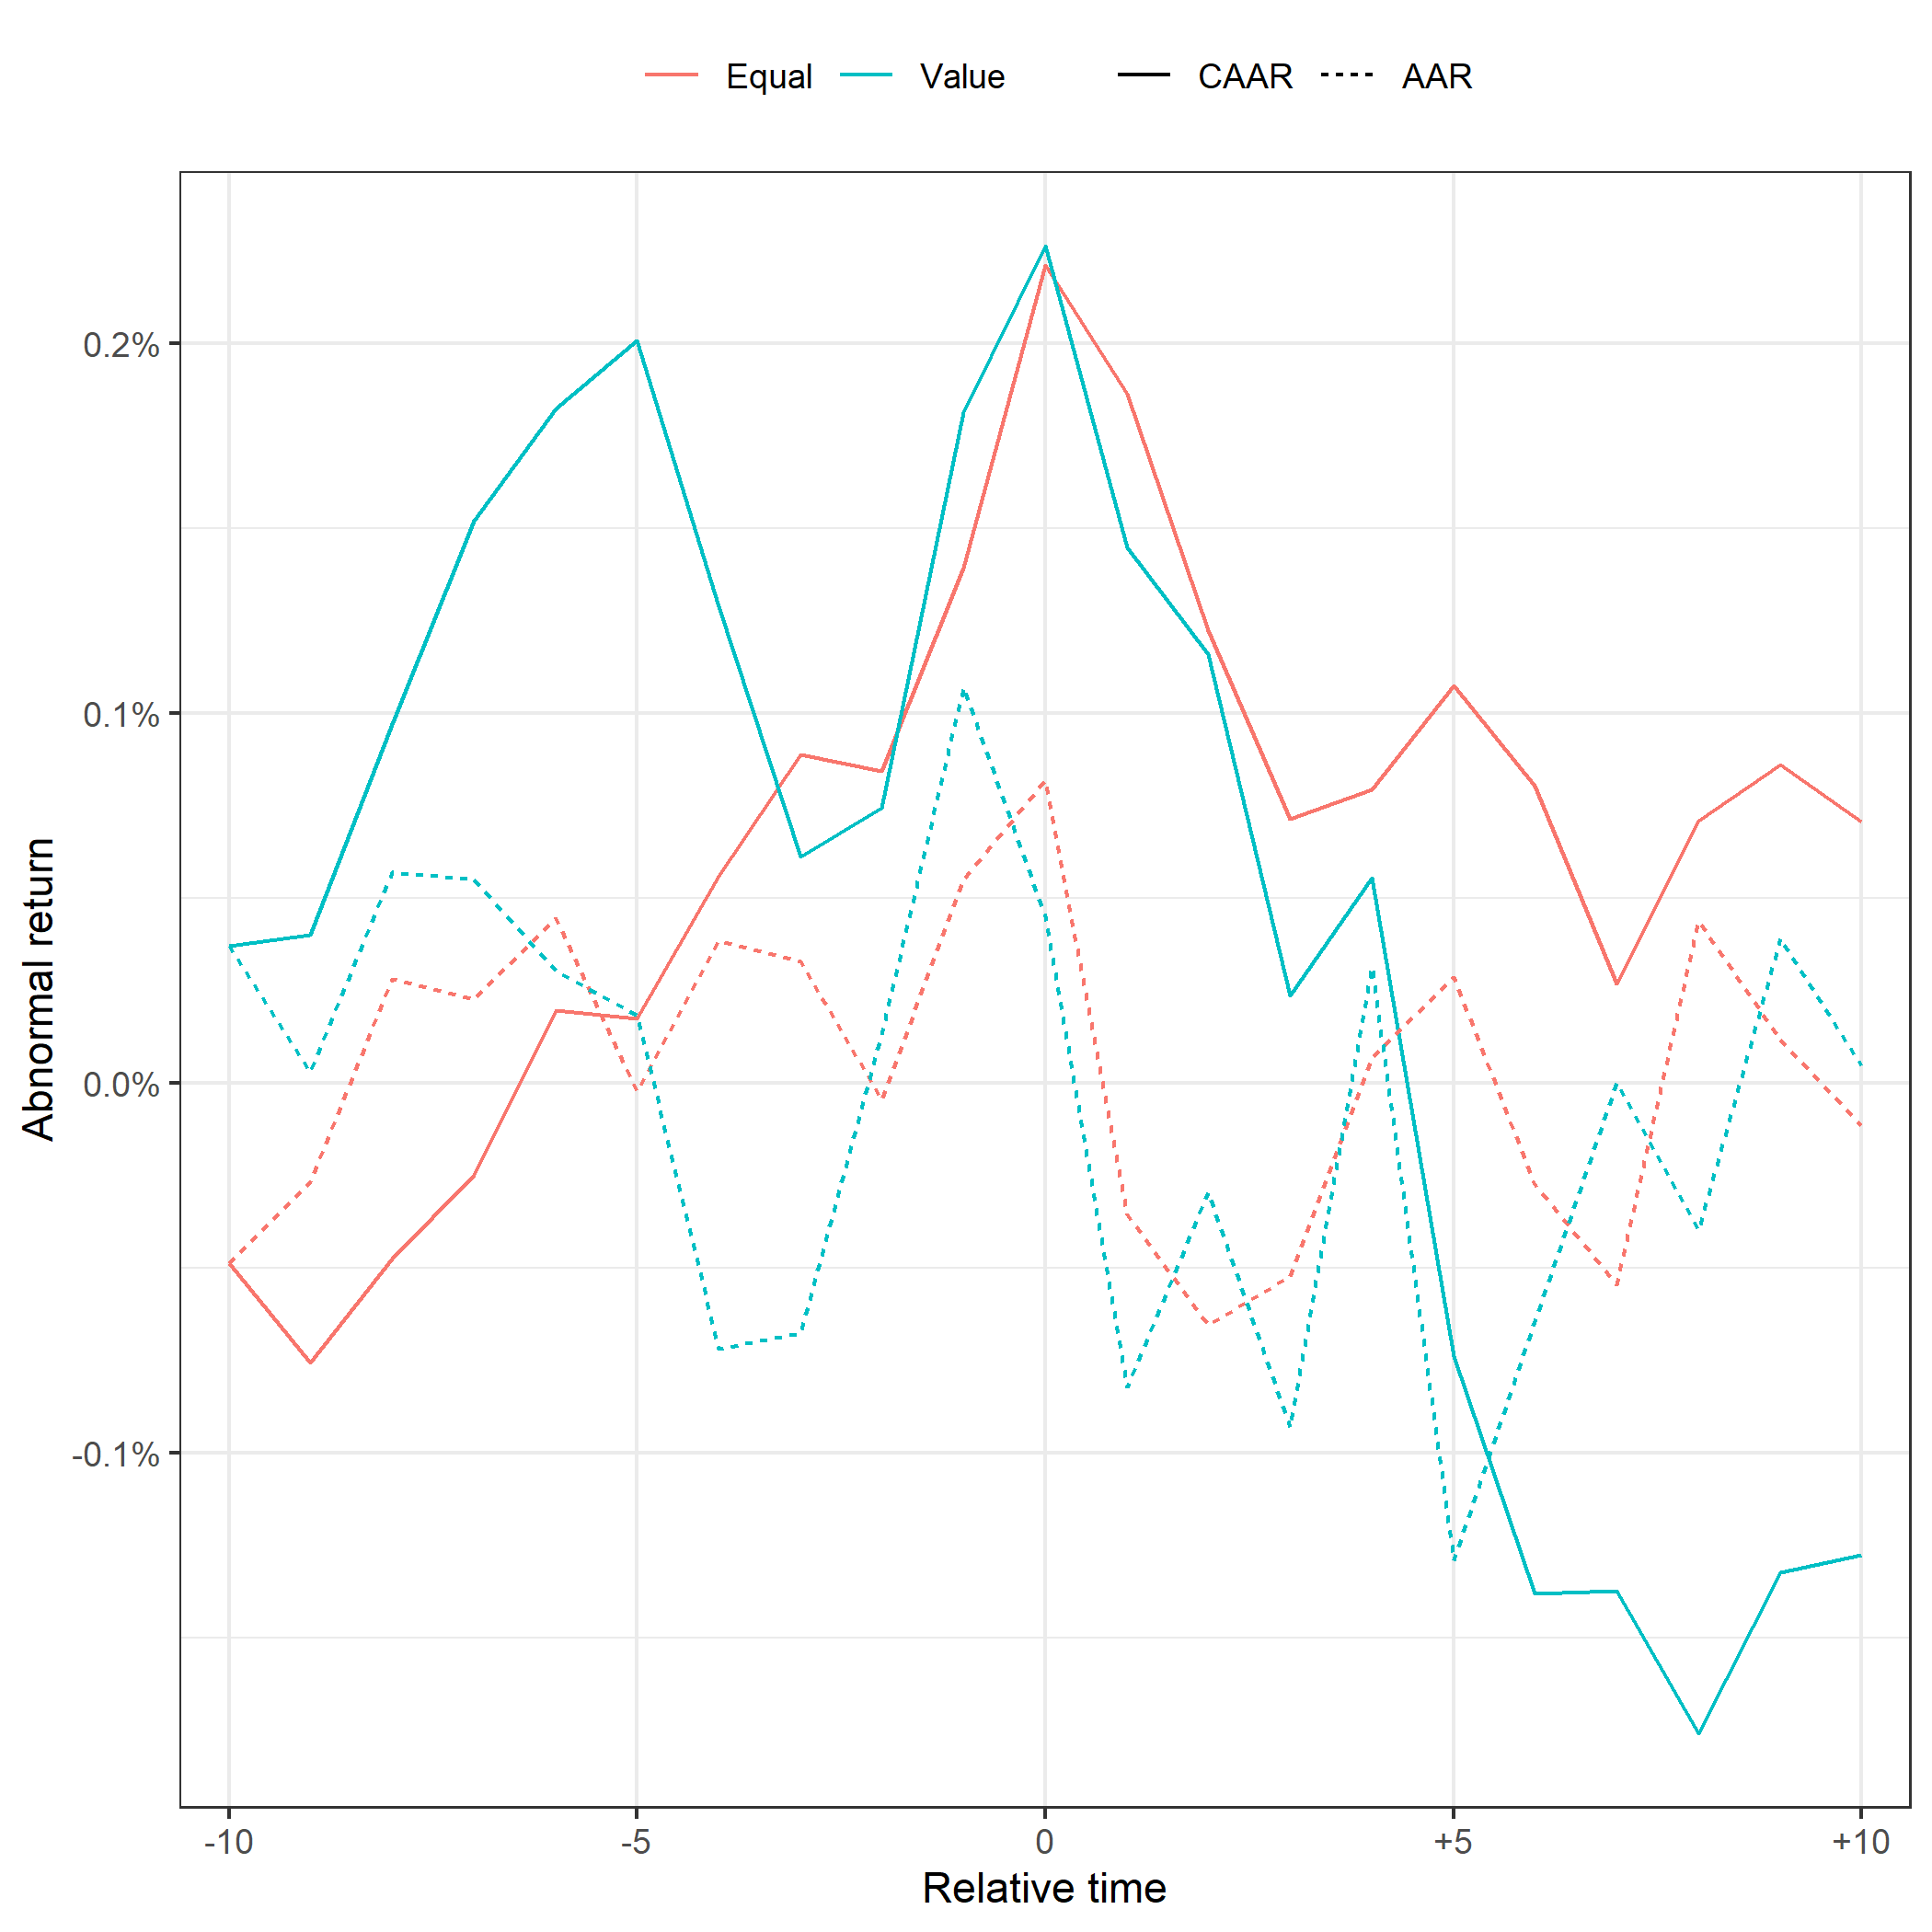
\includegraphics[scale=0.6]{Projekt/1.Figures analysis/ST_positive_sensitivity_weight.png}
     \caption*{\footnotesize The figure illustrates the average abnormal return (AAR) and cumulative AAR (CAAR) around the event date (t = 0) of positive news. The blue lines are returns calculated from an equally weighted portfolio, while the weights of the red lines are based on market capitalization. }
    \label{fig:ST_pos_sensitivity_weights}
\end{figure} 


\begin{table}[H]
\centering
\caption{AAR and CAAR (in \%) with equally weighted returns} 
\begin{tabular}{lcccc}
  \hline  \hline
  & \multicolumn{1}{c}{Positive} &  \multicolumn{1}{c}{Negative}\\  
 \hline
$AAR_{t=0}$ &  $\underset{(0.634)}{0.045}$ & $\underset{(-3.509)}{-0.378^{***}}$ \\  
$CAAR_{[-5;+5]}$  & $\underset{(-1.233)}{-0.258}$ & $\underset{(-4.4255)}{-0.858^{***}}$ \\ 
$CAAR_{[-10;+10]}$    & $\underset{(-0.452)}{-0.128 }$ & $\underset{(-3.012)}{-0.822^{***}}$ \\ 
   \hline \hline
   \multicolumn{3}{p{10cm}}{ \footnotesize $^* \; p\; <\; 0.1$, $ ^{**} \; p\; <\; 0.05$, $ ^{***} \; p\; <\; 0.01$  } \\
   \multicolumn{3}{p{10cm}}{\footnotesize The tables shows the CAAR associated with positive and negative news over an event window of 5, 10, and 21 days surrounding the event date along with the AAR on $t=0$. The models are split on the requirement rule for included events (2 or 3 sd).} \\
   \hline
\end{tabular}
\label{tab:ST_sensitivity_weights}
\end{table}

\subsubsection{Long term}

\begin{figure} [H]
     \centering
     \begin{minipage}[b]{0.49\textwidth}
         \centering
    \caption{Positive news: Nasdaq Global}
    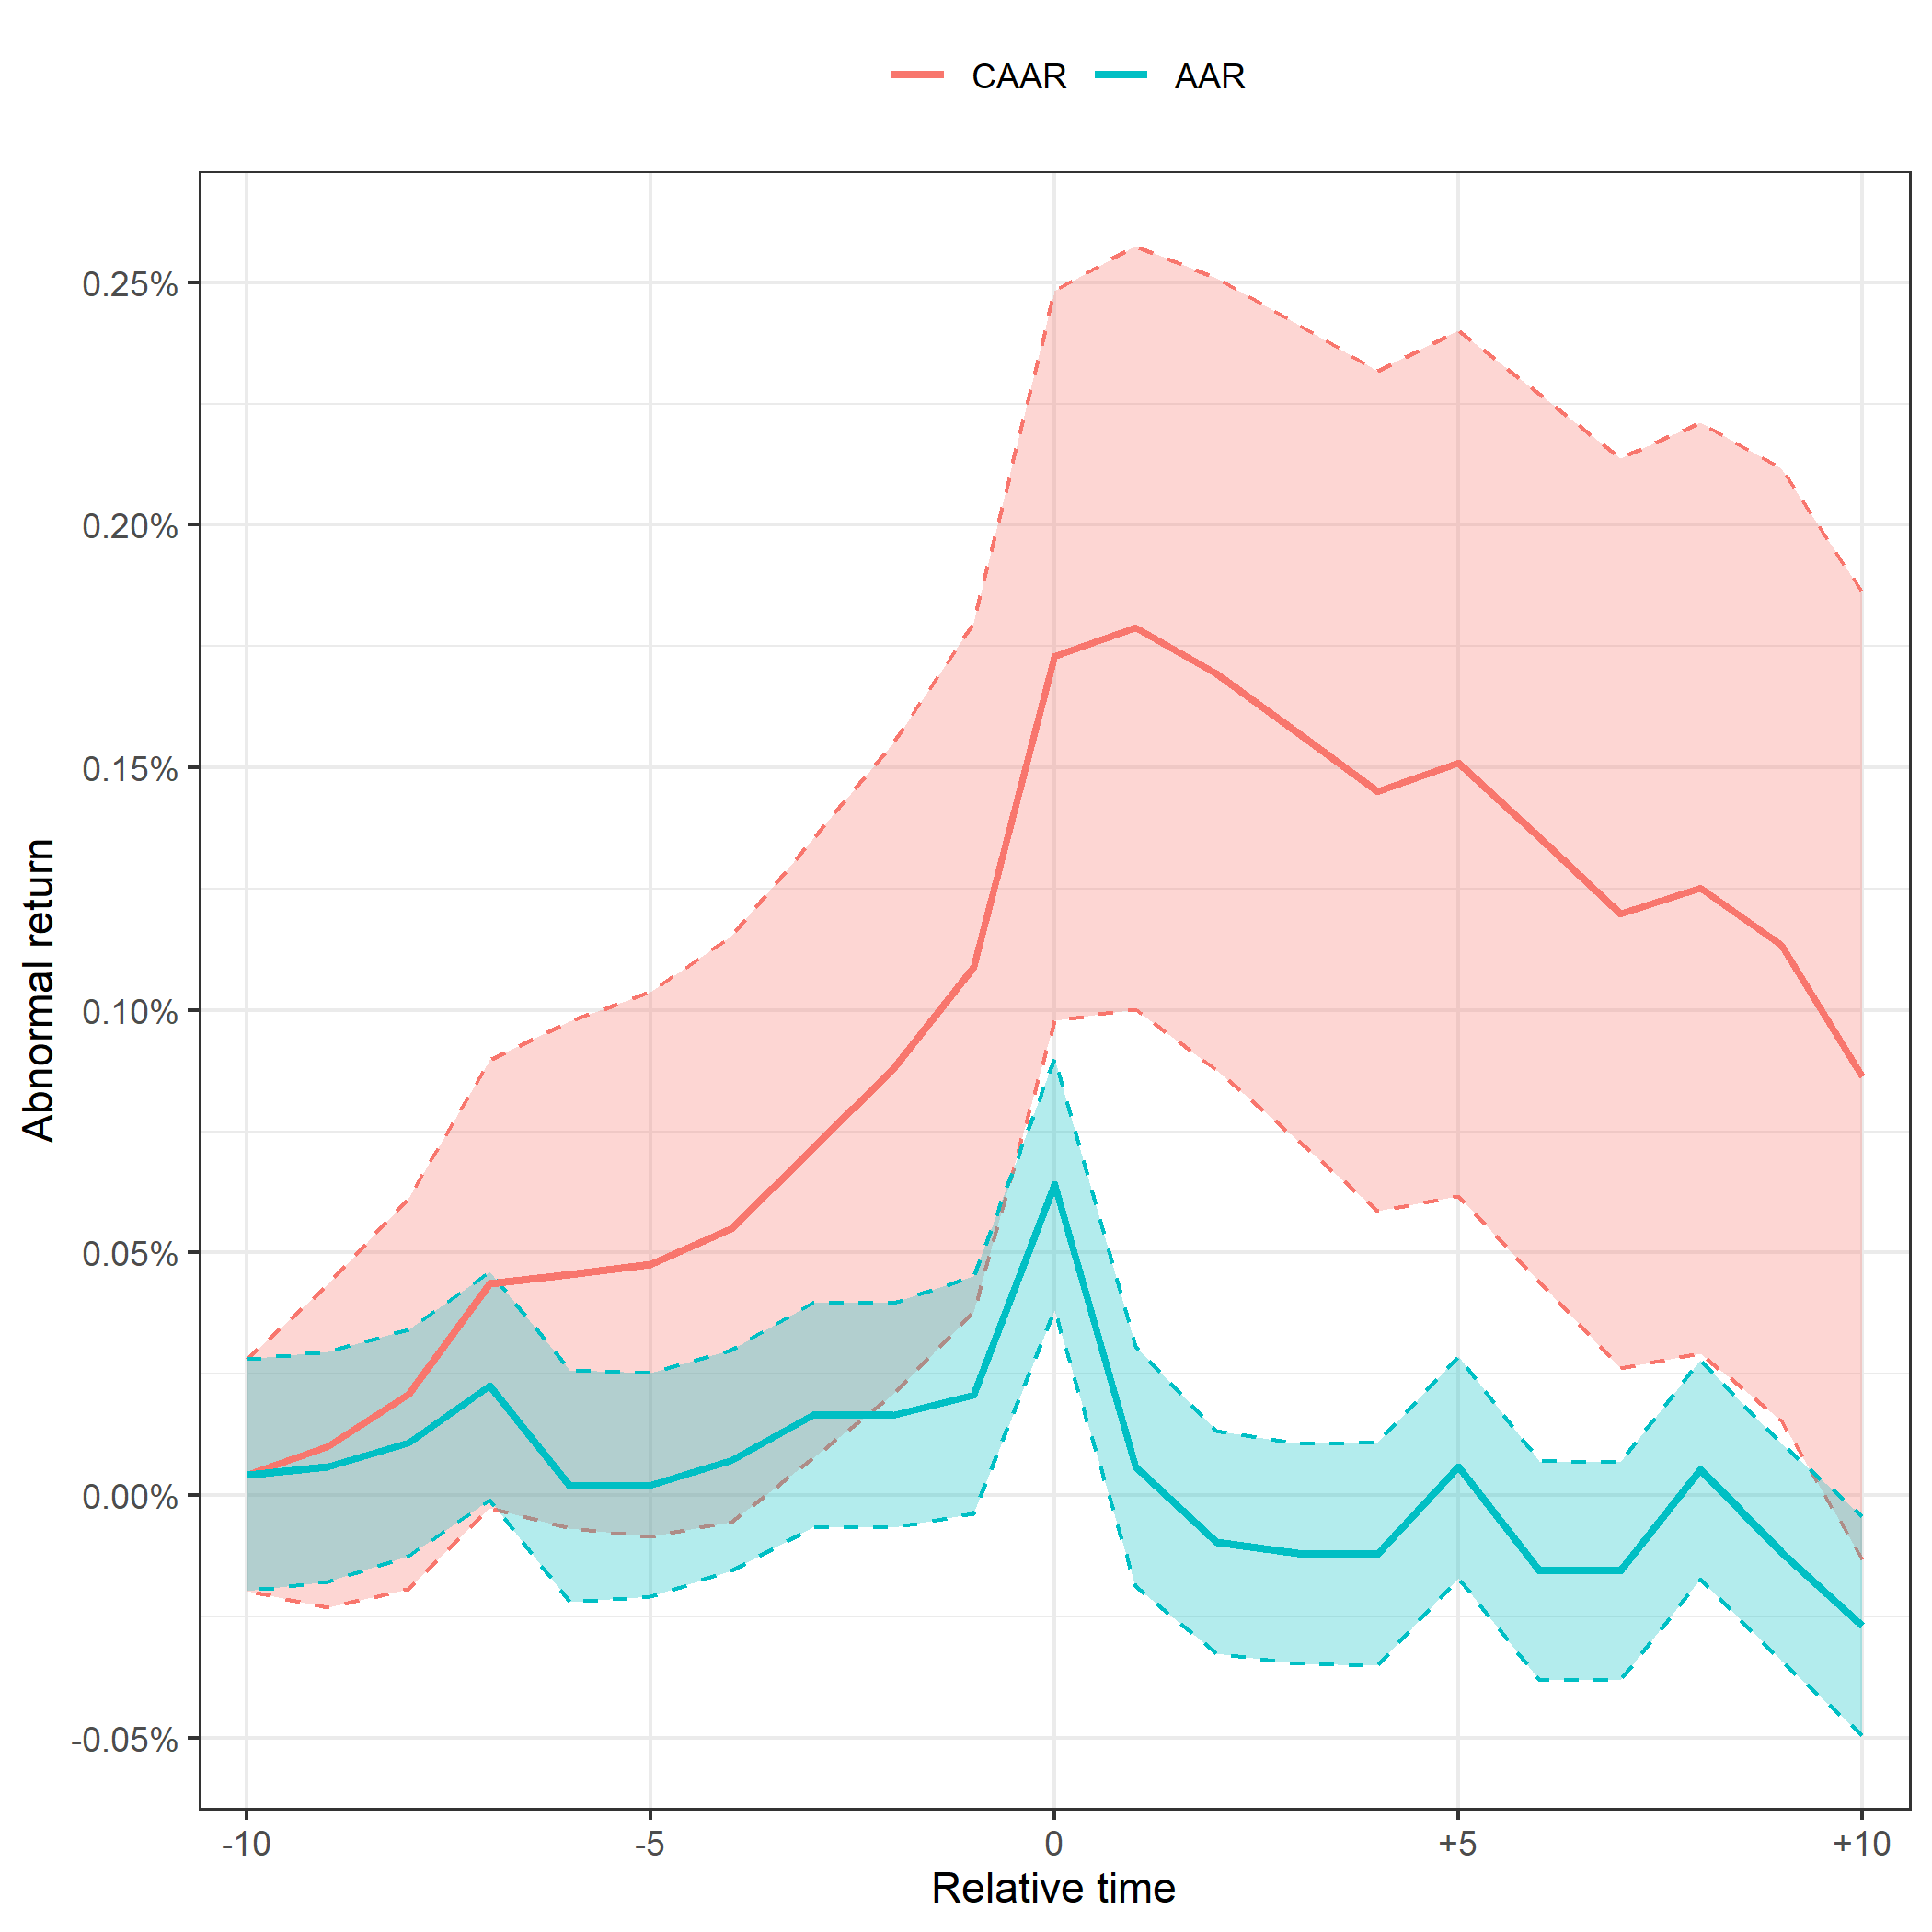
\includegraphics[width=\textwidth]{Projekt/1.Figures analysis/ST_positive_all_CI_nasdaq.png}
     \label{fig:ST_pos_sensitivity_nasdaq}
     \end{minipage}
     \hfill
     \begin{minipage}[b]{0.49\textwidth}
       \centering
    \caption{Positive news: Nasdaq Global, ESG}
    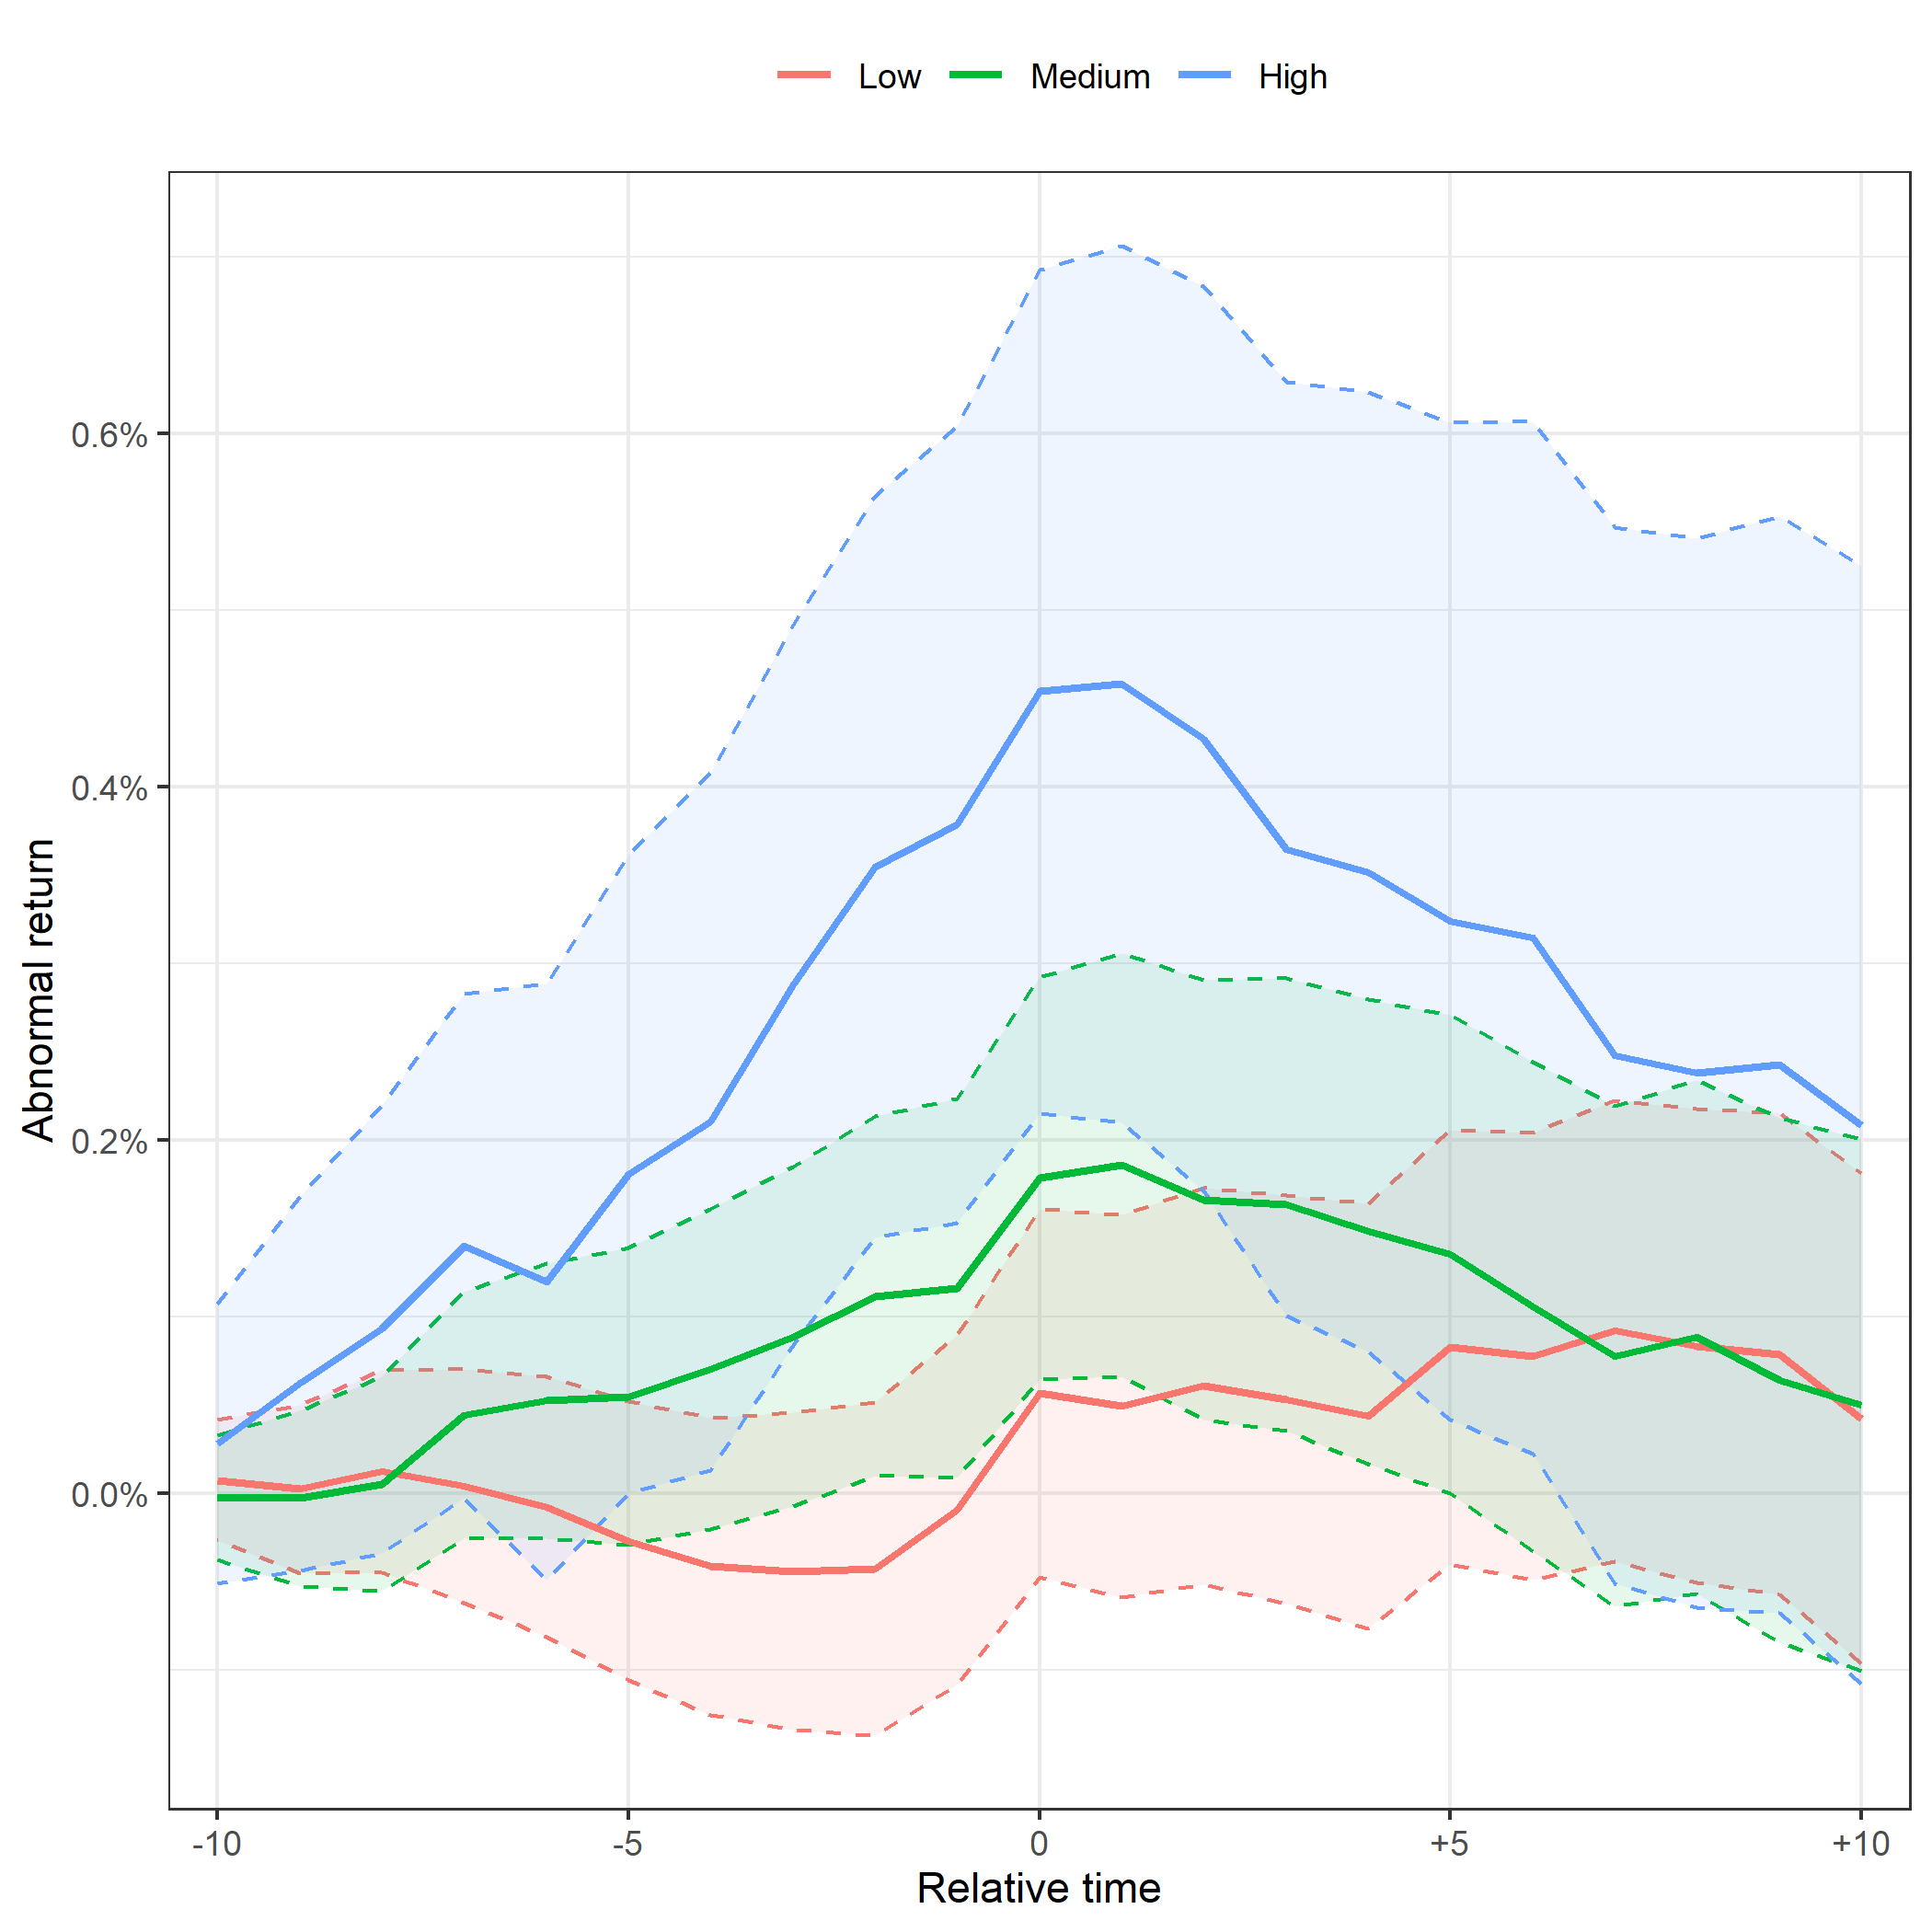
\includegraphics[width=\textwidth]{Projekt/1.Figures analysis/ST_positive_ESG_nasdaq.png}
    \label{fig:ST_pos_sensitivity_nasdaq_ESG}
     \end{minipage}
        \caption*{\footnotesize The figure illustrates the average abnormal return (AAR) and cumulative AAR (CAAR) around the event date (t = 0) of negative news. The blue lines are returns calculated from an equally weighted portfolio, while the red lines are based on market capitalization weights.}
        \label{fig:three graphs}
\end{figure}













\setlength{\tabcolsep}{15pt}
\begin{table}[]
\small
\centering
\caption{Fama-French five-factor model alpha from positive news with equal weights} 
\begin{tabular}{ccccc}
\hline \hline \\ 
 &     &  &    1 SD  & \\ \cline{3-4}
& & &  T = 1 & \\ \cline{3-4}
& Alpha (\%)  &  & $ -0.004$  &  \\
& t-value &  & -1.55 &  \\
& & &  T = 4 & \\ \cline{3-4}
& Alpha (\%)  &  & $ -0.003^{*}$  & \\
& t-value & & -1.77  &  \\
& & &  T = 8 & \\ \cline{3-4}
& Alpha (\%)  &  & $ -0.003^{***}$   &  \\
& t-value &  & -2.98  & \\
&  & &  T = 12 & \\ \cline{3-4}
& Alpha (\%)  &  & $ -0.004^{***}$  &  \\
& t-value &  & -3.02  & \\
\hline \hline
 \multicolumn{5}{l}{ \footnotesize $^* \; p\; <\; 0.1$, $ ^{**} \; p\; <\; 0.05$, $ ^{***} \; p\; <\; 0.01$  } \\
 \multicolumn{5}{p{11.5cm}}{ \footnotesize Alpha is the WLS-regression intercept (in \%) of the Fama-French 3-factor model, displayed along with the corresponding t-value. N is the average amount of firms included in the portfolio each month, and T is the portfolio holding period. The threshold for event firms to be included in the portfolio is either 1,2 or 3 "SD" (standard deviations) larger than the mean.}  \\ 
\end{tabular}
\label{tab: FF5_pos_equalW}
\end{table}


\setlength{\tabcolsep}{15pt}
\begin{table}[H]
\small
\centering
\caption{FF-5 model alpha from positive news with altered event identification rule } 
\begin{tabular}{ccc}
\hline \hline \\ 
&  2 SD  &  3 SD   \\ \cline{2-3} 
 \multicolumn{2}{c}{ T = 1}  \\ \hline
 Alpha (\%) & 0.04  & -0.37   \\
 t-value & 0.11  & -0.74  \\
 \multicolumn{2}{c}{ T = 4}  \\ \hline
 Alpha (\%)  & 0.03  &  -0.07  \\
 t-value  & 0.13  & -0.23  \\
 \multicolumn{2}{c}{ T = 8}  \\ \hline
 Alpha (\%) & -0.01  & 0.04   \\
 t-value & -0.15 & 0.18  \\
 \multicolumn{2}{c}{ T = 12}  \\ \hline
 Alpha (\%) & 0.13  & 0.23   \\
 t-value & 1.09 & 1.35  \\
 \hline \hline
 \multicolumn{3}{l}{ \footnotesize $^* \; p\; <\; 0.1$, $ ^{**} \; p\; <\; 0.05$, $ ^{***} \; p\; <\; 0.01$  } \\
 \multicolumn{3}{p{5cm}}{ \footnotesize Alpha is the WLS-regression intercept (in \%) of the Fama-French 5-factor model, displayed along with the corresponding t-value. N is the average amount of firms included in the portfolio each month, and T is the portfolio holding period. The threshold for event firms to be included in the portfolio is either 1,2 or 3 standard deviations (SD) larger than the mean.}  \\ 
\end{tabular}
\label{tab: FF5_pos}
\end{table}
